\documentclass[french]{template}

\usepackage{listings}

\begin{document}

\titre{Projet HagiMule}
\UE{Systèmes Concurrents et Communicants}
\enseignant{Daniel \textsc{Hagimont}}
\eleves{Leïlie \textsc{Canillac} \\ Vianney \textsc{Hervy}}


\fairemarges
\fairepagedegarde
\tabledematieres
\listedesfigures

\section{Introduction}

Le projet contient les éléments principaux suivants :
\begin{itemize}
    \item un annuaire qui enregistre les fichiers et les informations des fichiers des clients connectés,
    \item Un client qui permet de se connecter à un annuaire, de servir des fichiers et de les télécharger.
\end{itemize}

\section{Approches de la fragmentation et du parallélisme}

Notre approche initiale était de découper le fichier demandé en fragments de taille fixe, puis de distribuer ces fragments aux hôtes possédant le fichier, quitte à ce que plusieurs hôtes servent plusieurs fragments différents. Pour cela, il fallait créer une connection socket pour chaque fragment.

Notre approche finale est de découper le fichier en autant de fragments que d'hôtes possédant le fichier, puis de demander un fragment à chaque hôte. Ainsi, une seule connection socket TCP par hôte est nécessaire.

\section{Architecture globale}

Le projet est réparti en plusieurs packages :

\begin{itemize}
    \item \texttt{fr.n7.hagimule} : contient les classes utilitaires
    \item \texttt{fr.n7.hagimule.client} : contient les classes client
    \item \texttt{fr.n7.hagimule.client.daemon} : contient les classes relatives au démon
    \item \texttt{fr.n7.hagimule.client.downloader} : contient les classes relatives au téléchargeur
    \item \texttt{fr.n7.hagimule.client.gui} : contient les classes relatives à l'interface graphique du client
    \item \texttt{fr.n7.hagimule.diary} : contient les classes relatives à l'annuaire
    \item \texttt{fr.n7.hagimule.test} : contient les tests unitaires
\end{itemize}

\subsection{Annuaire}

Un annuaire est accessible via RMI\footnote{\url{https://en.wikipedia.org/wiki/Java_remote_method_invocation}}. Il lui faut donc un "serveur" qui réalise seulement le binding de l'annuaire. C'est la classe \texttt{DiaryServer}. L'annuaire lui-même est implémenté dans la classe \texttt{DiaryImpl}.

Lors des premières itérations, nous avons conçu l'annuaire de telle sorte à ce que toutes ses méthodes soient publiques. Après plusieurs réécritures et changements d'implémentation interne, nous avons décidé de spécifier clairement les méthodes dans une interface. Plus tard encore, avec l'apparition des connections persistantes, nous avons réalisé que certaines méthodes de l'annuaie devraient être uniquement accessibles par un client ou uniquement par un serveur. Nous avons donc créé deux interfaces : \texttt{ClientDiary} et \texttt{ServerDiary}. Elles spécifient chacunes un annuaire tel qu'il est vu par un client ou un serveur. Le diagramme de classes est visible sur la figure \ref{fig:diary}.

\begin{figure}[h]
    \centering
    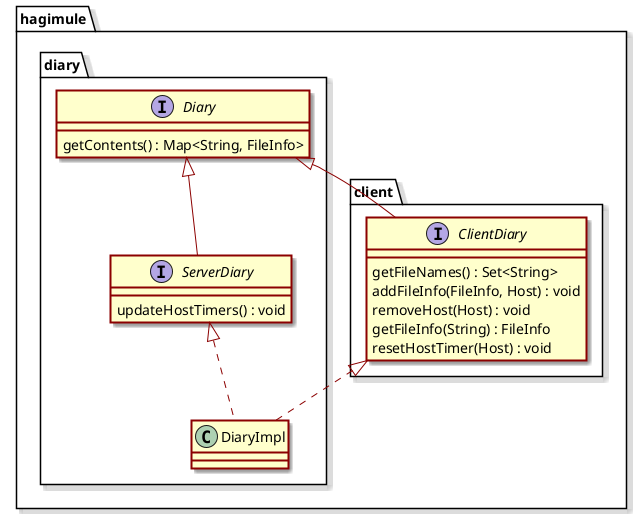
\includegraphics[width=1\textwidth]{img/diary.png}
    \caption{Diagramme de classes de l'annuaire}
    \label{fig:diary}
\end{figure}

\subsection{Client}

Un client (classe \texttt{Client}) a un démon (classe \texttt{Daemon}) et un téléchargeur (classe \texttt{Downloader}).

Un démon est toujours à l'écoute d'une connection TCP. Lorsqu'une connection est établie, il crée un esclave (classe \texttt{DaemonSlave}) qui va servir le fragment demandé. Cet esclave s'exécute dans un thread séparé et ne bloque donc pas le démon qui reste à l'écoute.

Un téléchargeur est un objet simple qui ne s'exécute pas dans un thread séparé. Sa méthode \texttt{downloadFile(String)} crée une tâche de téléchargement (classe \texttt{DownloadTask}) qui s'exécute dans un thread séparé. Cette classe de tâche gère l'ensemble de la logique pour le téléchargement d'un fichier. Elle récupère hôtes et crée les esclaves (classe \texttt{DownloaderSlave}) qui vont télécharger les fragments.

Un esclave de téléchargement est créé avec un hôte et des informations sur le fragment à télécharger. Il se connecte à l'hôte, lui demande le fragment, le reçoit et  l'écrit lui-même dans l'attribut (synchonized) \texttt{fileBytes} de sa tâche parente avec la méthode \texttt{writeFragment(byte[],int)}. Ainsi, la tâche de téléchargement n'est pas responsable de l'assemblage des fragments. Elle attends juste la terminaison de tous ses esclaves avant d'écrire le fichier sur le disque.

\section{Lancement en ligne de commande}

Un client et un serveur annuaire peuvent être lancés en ligne de commande (l'hébergeur peut vouloir fonctionner uniquement en mode démon). On peut spécifier des options en argument comme décrit dans les figures \ref{fig:diary-cli-doc} et \ref{fig:client-cli-doc}.

Lorsqu'un client est lancé, il va de suite essayer de se connecter à l'annuaire. Si l'annuaire n'est pas accessible, il réessaie en boucle toutes les 10 secondes. Dès que la connection est établie, il le signal à l'utilisateur et synchronise les fichiers servables.

\begin{figure}[h]
    \begin{lstlisting}
        usage: ./scripts/diary [--gui]
        -g,--gui    Run the server with a GUI
        -h,--help   Print this message
    \end{lstlisting}
    \caption{Documentation du lancement du serveur annuaire}
    \label{fig:diary-cli-doc}
\end{figure}

\begin{figure}[h]
    \begin{lstlisting}
    usage: ./scripts/client [-p <daemon port>] [-d <diary server IP>]
    -d,--diary <arg>   IP address of the diary server
    -g,--gui           Run the client with a GUI
    -h,--help          Show help
    -p,--port <arg>    Port number for the daemon
\end{lstlisting}
    \caption{Documentation du lancement du client}
    \label{fig:client-cli-doc}
\end{figure}

\section{Interfaces graphiques}

Les interfaces graphiques de ce projet ont été réalisées avec les packages \texttt{java.awt}\footnote{\url{https://en.wikipedia.org/wiki/Abstract_Window_Toolkit}} et \texttt{javax.swing}\footnote{\url{https://en.wikipedia.org/wiki/Swing_(Java)}}. Seuls les deux éléments principaux: le client et le serveur annuaire ont une interface graphique.

\subsection{Interface graphique serveur annuaire}

L'interface graphique du serveur annuaire (figure \ref{fig:server-gui}) ne sert qu'à l'affichage des fichiers servables et des hôtes connectés, on ne peut pas interagir avec.

\begin{figure}[h]
    \centering
    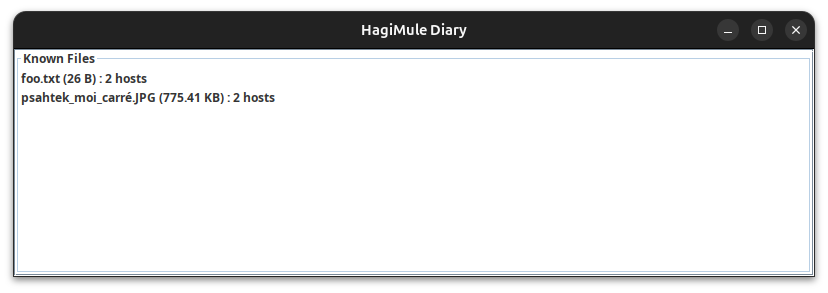
\includegraphics[width=1\textwidth]{img/diary-gui.png}
    \caption{Interface graphique du serveur annuaire}
    \label{fig:server-gui}
\end{figure}

\subsection{Interface graphique client}

L'interface graphique du client (figure \ref{fig:client-gui}) a été réalisée assez tôt dans leprojet car il étatait nécessaire d'interagir avec le client pour tester les fonctionnalités. Elle permet de choisir l'IP du serveur annuaire, de lister les fichiers servables et d'en télécharger un. Les téléchargements en court son affichés dans le rectangle inférieur.

\begin{figure}[h]
    \centering
    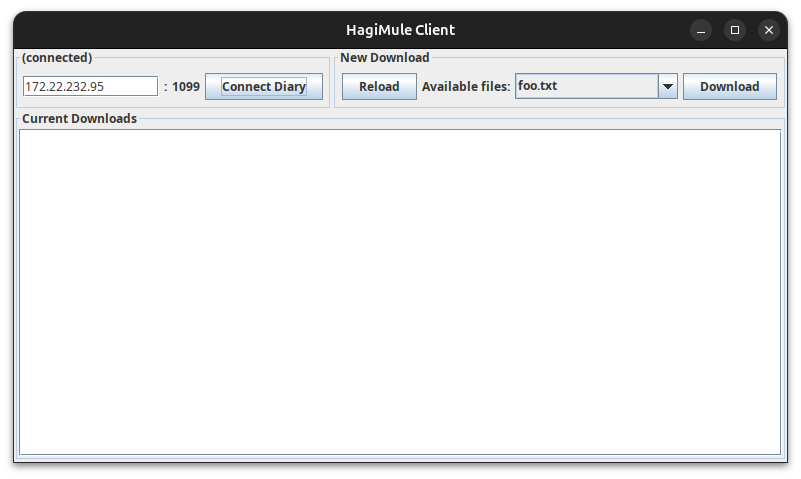
\includegraphics[width=1\textwidth]{img/client-gui.png}
    \caption{Interface graphique du client}
    \label{fig:client-gui}
\end{figure}

\section{Synchronisation annuaire / démon}

\subsection{Connection persistante}

Un des enjeux du projet est d'avoir un annuaire à jour. Pour cela, nous avons mis en place un système de connection dite "keep-alive" entre le démon et l'annuaire.

L'annuaire possède pour chaque hôte dont il a connaissance un timer. Chaque seconde, le serveur hébergeant l'annuaire décrémente ce timer. Si le timer atteint 0, l'annuaire considère l'hôte associé comme inaccessible et le supprime de sa liste.

Le démon quant à lui, a accès via RMI à une méthode \texttt{resetHostTimer(Host)} qui remet à 3 le timer de l'hôte passé en paramètre (lui-même). Nous avons fait le choix de créer un thread qui appelle cette méthode à chaque seconde plutôt que de l'appeler à chaque fois que le démon effectue une action.

\subsection{Fichiers servables}

Il n'est pas seulement nécessaire de synchroniser l'accessibilité des hôtes, mais aussi les fichiers qu'ils servent. Pour cela, nous avons implémenté une méthode de surveillance des fichiers servables avec l'aide du package \texttt{java.nio.file}. Cette surveillance effecture une sychronisation avec l'annuaire chaque fois qu'un fichier est ajouté, supprimé ou modifié.

\subsection{Obstacles rencontrés}

La conception des solutions de synchronisation était plutôt directe et simple, mais ce qui a posé problème était la gestion des accès concurrents à l'annuaire. La solution était donc de marquer les méthodes de l'annuaire comme \texttt{synchronized}.

\section{Code}

L'ensemble du code est compatible avec Java 11\footnote{\url{https://openjdk.java.net/projects/jdk/11/}}.

Le code est en partie documenté suivant les conventions Javadoc\footnote{\url{https://docs.oracle.com/javase/8/docs/technotes/tools/windows/javadoc.html}}. Des commentaires sont présents lorsque le code n'est pas suffisamment clair.

Des tests ont été réalisé tout au long du développement. Vous trouverez ainsi des suites de tests JUnit\footnote{\url{https://junit.org/}} dans le package \texttt{fr.n7.hagimule.test}. Ceux-ci n'ont pas été mis-à-jour en fin de développement et ne sont pas garantis de passer ni même de compiler.

\subsection{Dépendances}

Le projet utilise trois dépendances externes au JDK :
\begin{itemize}
    \item \texttt{org.apache.commons.cli}\footnote{\url{https://commons.apache.org/proper/commons-cli/}} pour la gestion des arguments de la ligne de commande lors du lancement d'un client ou du serveur annuaire,
    \item \texttt{org.junit}\footnote{\url{https://junit.org/}} pour les tests unitaires,
    \item \texttt{org.hamcrest}\footnote{\url{https://hamcrest.org/}} pour les tests unitaires.
\end{itemize}

\section{Exigences non satisfaites}

\begin{itemize}
    \item \textbf{Robustesse}: Si un hôte se déconecte, supprime son fichier ou que le fragment se perd, le téléchargement échoue, il n'y a pas de tentative de reconnection.
    \item \textbf{Optimisation}: Le téléchargeur ne prend pas en compte l'occupation des sources lors de la répartition des fragments.
    \item \textbf{Compression}: Ni les fragments individuels, ni les fichiers ne sont compressés. Chaque octet est envoyé tel qu'écrit sur le disque de l'hôte.
\end{itemize}

\section{Améliorations possibles}

En plus des exigences non satisfaites, voici quelques améliorations possibles :

\begin{itemize}
    \item \textbf{Robustesse}: Implémenter un système de clé sha256 pour différentier les fichiers servis, plutôt que de se baser sur le nom du fichier. Cela permettrait de vérifier l'intégrité d'un fichier téléchargé.
    \item \textbf{Optimisation}: Permettre l'écriture sur disque d'un fragment même lorsque le fichier complet n'a pas été téléchargé. Cela diminuerait l'utilisation de la mémoire vive en cas de téléchargement de gros fichiers.
\end{itemize}

\section{Annexes}

\begin{figure}[h]
    \centering
    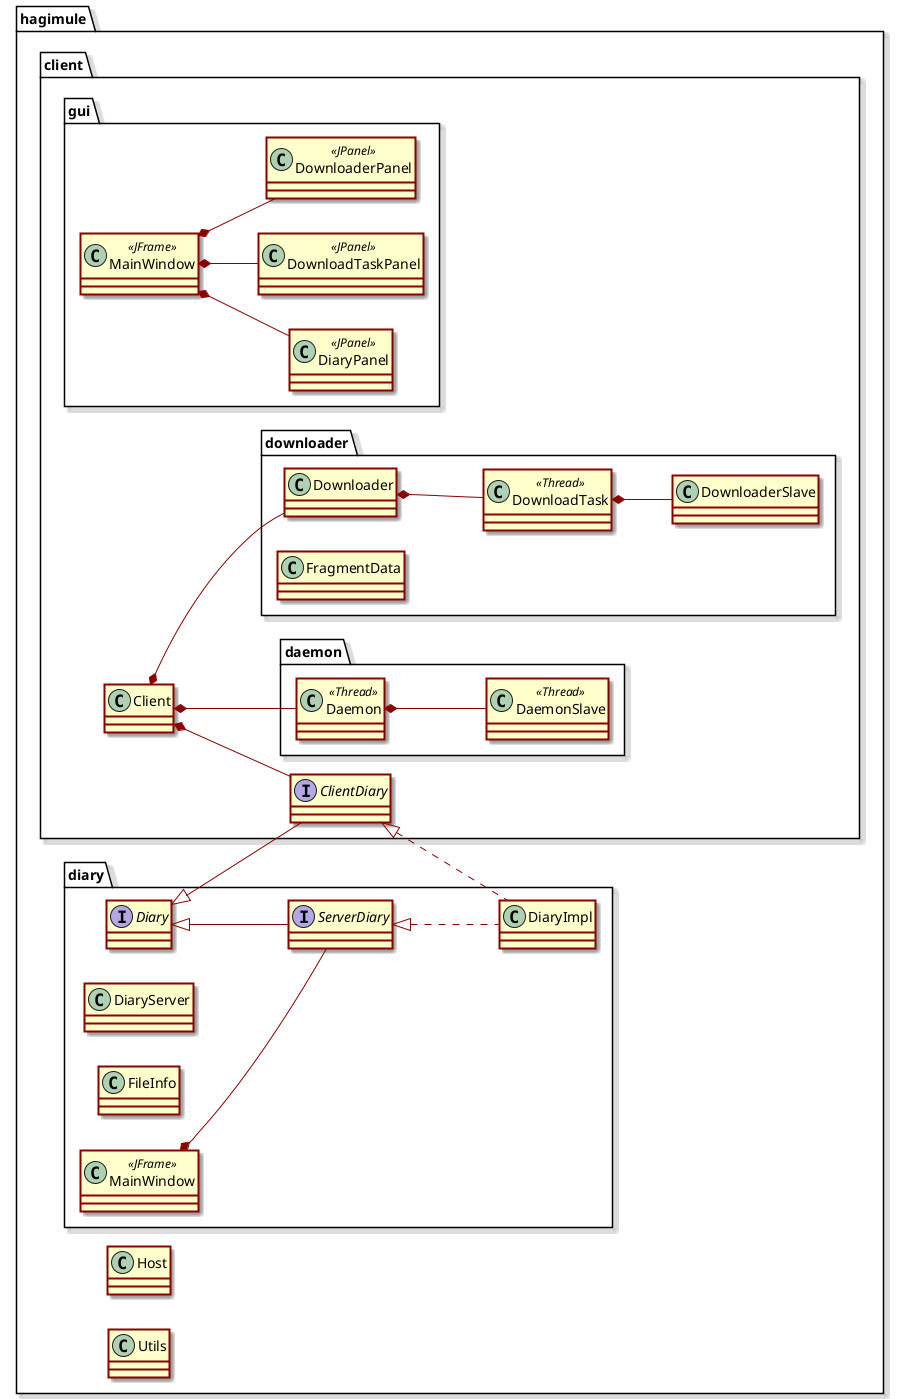
\includegraphics[width=0.9\textwidth]{img/archi.png}
    \caption{Diagramme de classes global simplifié}
    \label{fig:diary}
\end{figure}

\end{document}